\documentclass{article}
\usepackage[utf8]{inputenc}
\usepackage{graphicx}

\title{CIRCLES}

\begin{document}

\maketitle
1.) If A and B are points in the plane such that PA/PB = k(constant) for all P on a given circle, then the value of k cannot be equal to..............

\vspace{5mm}
2.) The points of intersection of the line 4x-3y-10=0 and the circle $x^2+y^2-2x+4y-20 = 0$ are............... and ................

\vspace{5mm}
3.)   The lines 3x-4y+4=0 and 6x-8y-7=0 are tangents to the same circle. The radius of the circle is.............

\vspace{5mm}
4.)   Let $x^2+y^2-4x-2y-11=0$ be circle. A pair of tangents (4,5) with a pair radii from quadrilateral of area..............

\vspace{5mm}
5.) From the origin chords are drawn to the circle $(x-1)^2+y^2=1$. The equation of the locus of the mid-points of these chords is............

\vspace{5mm}
6.) The equation of the line passing through the points of intersection of the circles $3x^2+3y^2-2x+12y-9=0$ and $x^2+y^2+6x+2y-15=0$ is................

\vspace{5mm}
7.) From the point A(0,3) on the circle $x^2+4x+(y-3)^2=0$, a chord AB is drawn and extended to a point M such that AM=2AB.The equation of the locus of M is..............

\vspace{5mm}
8.) The area of the triangle is formed by tangents from the point (4,3) to the circle $x^2+y^2=9$ and the line joining their points of contact is........... 

\vspace{5mm}
9.) If the circle $C_1:x^2+y^2=16$ intersects another circle $C_2$ of radius 5 in such a manner that common chord is of maximum length and has a slope equal to 3/4, then the coordinates of the centre $C_2$ are...........

\vspace{5mm}
10.) The area of the triangle formed by the positive x-axis and the normal and the tangent to the circle $x^2+y^2=4$ at (1,\sqrt{3})       is...............

\vspace{5mm}
11.) If a circle passes through the points of intersection of the coordinate axes with the lines kx-y+1=0 and x-2y+3=0, then the value of k=..............

\vspace{5mm}
12.) The equation of the locus of the midpoints of the circle $4x^2+4y^2-12x+4y+1=0$ that subtend of a angle of 2$\pi_{}/3$  at its centre is..............

\vspace{5mm}
13.) The intercept on the line y=x by the circle $C1:x^2+y^2-2x=0$ is AB.Equation of the circle with AB as a diameter is...............

\vspace{5mm}
14.) For each natural number k, let $C_k$ denote the circle with radius k centimetres and center at origin. On the circle $C_k$, $\alpha_{}$-particle moves k centimetres in the counter clockwise direction. After completing its motion on $C_k$ the particle moves to $C_{k+1}$ in the radial direction. The motion of the particle is continues in the manner. The particle starts at (1,0). If the particle crosses the positive direction of the x-axis for the first time on the circle $C_n$ then n=................

\vspace{5mm}

15.) The chords of contact of the pair of tangents drawn from each point on the line 2x+y=4 to circle $x^2+y^2=1$ pass through the point............


\section{True/False}

  1.) No tangent can be drawn from the point (5/2,1) to the circum circle of the triangle with vertices (1,\sqrt{3}), (1,-\sqrt{3}),  (3,-\sqrt{3}).
  
  \vspace{5mm}
2.) The line x+3y=0 is diameter of the circle $x^2+y^2-6x+2y=0$ 

\section{MCQs with One Correct Answer}

1.) A square is inscribed in the circle  $x^2+y^2-2x+4y+3=0$. Its sides are parallel to the coordinate axes. The one vertex of the square is

\choice  A. (1+\sqrt{2},-2)

\choice  B. (1-\sqrt{2},-2)

\choice  C. (1, -2+\sqrt{2},)

\choice  D. none of these

\vspace{5mm}
2.) The circles $x^2+y^2=6$ and  $x^2+y^2-2x+4y+3=0$ are given. Then the equation of the circle through their points of intersection and the point (1,1) is

\choice  A. $x^2+y^2-6x+4=0$

\choice  B. $x^2+y^2-3x+1=0$

\choice  C. $x^2+y^2-4y+2=0$

\choice  D. none of these

\vspace{5mm}
3.) The centre of the circle passing through the point (0,1) and touching the curve $y=x^2$ at (2,4) is

\choice  A. (-16/5, 27/10)

\choice  B. (-16/7, 53/10)

\choice  C. (-16/5, 27/10)

\choice  D.  none of these

\vspace{5mm}
4.) The equation of the circle passing through the point (1,1) and the points of intersection of $x^2+y^2+13x-3y=0$ and $2x^2+2y^2+4x-7y-25=0$ is 

\choice  A. $4x^2+4y^2-30x-10y-25=0$

\choice  B. $4x^2+4y^2+30x-13y-25=0$

\choice  C. $4x^2+4y^2-17x-10y+25=0$

\choice  D.  none of these

\vspace{5mm}
5.) The locus of the mid point of a chord of the circle $x^2+y^2=4$ which subtends a right angle at the origin is

\choice  A. x+y=2

\choice  B. $x^2+y^2=1$

\choice  C. $x^2+y^2=2$

\choice  D. x+y=1

\vspace{5mm}
6.) If a circle passes through the point (a,b) and cuts the circle $x^2+y^2=k^2$ orthogonally, then the equation of the locus of its centre is  

\choice  A. 2ax+2by-$(a^2+b^2+k^2)$=0

\choice  B. 2ax+2by-$(a^2-b^2+k^2)$=0

\choice  C. $x^2+y^2-3ax-4by+(a^2+b^2-k^2)=0$

\choice  D. $x^2+y^2-2ax-3by+(a^2-b^2-k^2)=0$

\vspace{5mm}
7.) If the two circles $(x-1)^2+(y-1)^2=r^2$ and $x^2+y^2-8x+2y+8=0$ intersect in two distinct points, then

\choice  A. $2 < r< 8$

\choice  B. $r < 2$

\choice  C. r=2

\choice  D. $r > 2$

\vspace{5mm}
8.) The lines 2x-3y=5 and 3x-4y=7 are diameters of a circle of area 154 sq.units. Then the equation of this circle is

\choice  A. $x^2+y^2+2x-2y=62$

\choice  B. $x^2+y^2+2x-2y=47$

\choice  C. $x^2+y^2-2x+2y=47$

\choice  D. $x^2+y^2-2x+2y=62$

\vspace{5mm}
9.) The centre of a circle passing through the points (0,0),(1,0) and touching the circle $x^2+y^2=9$  is

\choice  A. (3/2, 1/2)

\choice  B. (1/2, 3/2)

\choice  C. (1/2, 1/2)

\choice  D. (1/2, $(-2)^ 1/2$)

\vspace{5mm}
10.) The locus of the centre of a circle , which touches externally the circle $x^2+y^2-6x-6y+14=0$ and also touches the y-axis, is given by the equation:

\choice  A. $x^2-6x-10y+14=0$

\choice  B. $x^2-10x-6y+14=0$

\choice  C. $y^2-6x-10y+14=0$

\choice  D. $y^2-10x-6y+14=0$

\vspace{5mm}
11.) The circles $x^2+y^2-10x+16=0$ and $x^2+y^2=r^2$ intersect each other in two distinct points if

\choice  A. $ r< 2 $

\choice  B. $ r > 8 $

\choice  C. $ 2 < r < 8 $

\choice  D. $ 2 \leq r \leq  8 $

\vspace{5mm}
12.) The angle between a pair of tangents drawn  from a point P  to the circle $x^2+y^2+4x-6y+9\sin ^2(\alpha )+13\cos^2(\alpha )=0$ is 2$\pi_{}$. The equation of the locus of the point P is 

\choice  A. $x^2+y^2+4x-6y+4=0$

\choice  B. $x^2+y^2+4x-6y-9=0$

\choice  C. $x^2+y^2+4x-6y-4=0$

\choice  D. $x^2+y^2+4x-6y+9=0$

\vspace{5mm}
13.) If two distinct chords drawn from the point (p,q) on the circle $x^2+y^2=px+qy$ (where pq\neq0) are bisected by the x-axis, then

\choice  A. $p^2=q^2$

\choice  B. $p^2=8q^2$

\choice  C. $p^2 < 8q^2$

\choice  D. $p^2 > 8q^2$

\vspace{5mm}
14.) The triangle PQR is inscribed in the circle $x^2+y^2=25$. If Q and  R have co-ordinates (3,4) and (-4,3) respectively, then \angle QPR  is equal to

\choice  A.$\pi_{}$/2

\choice  B. $\pi_{}$/3

\choice  C. $\pi_{}$/4

\choice  D. $\pi_{}$/6

\vspace{5mm}
15.) If the circles $x^2+y^2+2x+2ky+6=0$, $x^2+y^2+2ky+k=2$ intersect orthogonally, then k is

\choice  A. 2 or -3/2

\choice  B. -2 or -3/2

\choice  C. 2 or 3/2

\choice  D. -2 or 3/2

\vspace{5mm}
16.) Let AB be chord of the circle $x^2+y^2=r^2$ subtending a right angle at at the centre. Then the locus of the centroid of the triangle PAB as P moves on the circle is

\choice  A. a parabola

\choice  B. a circle

\choice  C. a ellipse

\choice  D. a pair of straight lines

\vspace{5mm}
17.) Let PQ and RS be tangents at the extremities of the diameter PR of a circle of radius r. If PS and RQ intersect at a point on the circumference of the circle, then 2r equals

\choice  A. \sqrt{PQ.RS}

\choice  B. (PQ+RS)/2

\choice  C. 2PQ.RS/(PQ+RS)

\choice  D.  \sqrt{ ($ PQ^2+RS^2 $) }/2

\vspace{5mm}
18.) If the tangent at the point P on the circle $x^2+y^2+6x+6y-2=0$ meets a straight line 5x-2y+6=0 at a point Q on the y-axis then the length of PQ is

\choice  A. 4

\choice  B. 2\sqrt{5}

\choice  C. 5

\choice  D.  3\sqrt{5}

\vspace{5mm}
19.) The centre of the circle inscribed in square formed by the lines $x^2-8x+12=0$ and $y^2-14y+45=0$, is

\choice  A. (4,7)

\choice  B. (7,4)

\choice  C. (9,4)

\choice  D. (4,9)

\vspace{5mm}
20.) If one of the diameter of the circle $x^2+y^2-2x-6y+6=0$ is a chord to the circle with centre (2,1). then the radius of the circle is 

\choice  A. \sqrt{3}

\choice  B. \sqrt{2}

\choice  C. 3

\choice  D.  2

\vspace{5mm}
21.) A circle is given by $x^2+(y-1)^2=1$, another circle C touches it externally and also the x-axis, then the locus of its centre is

\choice  A. {(x,y):x^2=4y} \cup  {(x,y):y\leq0}

\choice  B. {(x,y):x^2+(y-1)^2=4} \cup  {(x,y):y\leq0}

\choice  C. {(x,y):x^2=y} \cup  {(0,y):y\leq0}

\choice  D.  {(x,y):x^2=4y} \cup  {(0,y):y\leq0}

\vspace{5mm}
22.) Tangents drawn from the point P(1,8) to the circle $x^2+y^2-6x-4y-11=0$ touch the circle at the points A and B.The equation of the circumcircle of the triangle PAB is

\choice  A. $x^2+y^2+4x-6y+19=0$

\choice  B. $x^2+y^2-4x-10y+19=0$

\choice  C. $x^2+y^2-2x+6y-29=0$

\choice  D.  $x^2+y^2-6x-4y+19=0$

\vspace{5mm}
23.) The circle passing through the point (-1,0) and touching the y-axis at(0,2) also passes through the point.

\choice  A. (-3/2, 0)

\choice  B. (-5/2, 2)

\choice  C. (-3/2, 5/2)

\choice  D. (-4,0)

\vspace{5mm}
24.) The locus of the mid-point of the chord of contact of tangents drawn from points lying on the straight line 4x-5y=20 to the circle $x^2+y^2=9$ is

\choice  A. 20(x^2+y^2)-36x+45y=0

\choice  B. 20(x^2+y^2)+36x-45y=0

\choice  C. 36(x^2+y^2)-20x+45y=0

\choice  D. 36(x^2+y^2)+20x-45y=0

\vspace{5mm}
25.) A line y=mx+1 intersects the circle $(x-3)^2+(y+2)^2= 25$ at the points P and Q. If the mid point of the line segment PQ has x-coordinate -3/5, then which one of the following option is correct?

\choice  A. $  2 \leq m <  4 $

\choice  B. $ -3 \leq m < -1 $

\choice  C. $  4 \leq m <  6 $

\choice  D. $  6 \leq m <  8$

\section{MCQs with One or More than One Correct}
\vspace{5mm}
1.) The equations of the tangents drawn from the origin to the circle  $x^2+y^2-2rx-2hy+h^2=0$, are

\choice  A. x=0

\choice  B. y=0

\choice  C. (h^2-r^2)x-2rhy=0

\choice  D. (h^2-r^2)x+2rhy=0

\vspace{5mm}
2.) The number of common tangents to the circles $x^2+y^2=4$ and $x^2+y^2-6x-8y=24$ is

\choice  A. 0

\choice  B. 1

\choice  C. 3

\choice  D. 4

\vspace{5mm}
3.) If the circle $x^2+y^2=a^2$ intersects the hyperbola $xy=c^2$ in four points P(x_1,y_1),Q(x_2,y_2),R(x_3,y_3),S(x_4,y_4), then

\choice  A. x_1+x_2+x_3+x_4=0

\choice  B. y_1+y_2+y_3+y_4=0

\choice  C. x_1x_2x_3x_4=c^4

\choice  D. y_1y_2y_3y_4=c^4

\vspace{5mm}
4.) Circles touching the x-axis at a distance 3 from the origin and having an intercept of length 2\sqrt{7}    on y-axis are 

\choice  A. $x^2+y^2-6x+8y+9=0$

\choice  B. y_1+y_2+y_3+y_4=0

\choice  C. x_1x_2x_3x_4=c^4

\choice  D. y_1y_2y_3y_4=c^4

\vspace{5mm}
5.) A circle S passes through the points (0,1) and is orthongonal to the circles $(x-1)^2+y^2=16$ and $x^2+y^2=1$.Then  

\choice  A. radius of S is 8

\choice  B. radius of S is 7

\choice  C. radius of S is (-7,1)

\choice  D. radius of S is (-8,1)

\vspace{5mm}
6.) Let RS be the diameter of the circle $x^2+y^2=1$ where S is the point (1,0).Let P be a variable point on the circle and tangents to the circle at S and P meet at the poitnt Q.The normal to the circle at P intersects a line drawn through Q parallel to RS at point E.Then the locus of E passes through the points 

\choice  A. (1/3, 1/\sqrt{3})

\choice  B.  (1/4, 1/2)

\choice  C.  (1/3, -1/\sqrt{3})

\choice  D.  (1/4, -1/2)

\vspace{5mm}

\section{Subjective Problems}

1.) Find the equation of the circle whose radius is 5 and which touches the circle $x^2+y^2-2x-4y-20=0$ at the point (5,5).

\vspace{5mm}
2.) Let AB be the centre of the circle $x^2+y^2-2x-4y-20=0$. Suppose that the tangents at the points of B(1,7) and D(4,-2) on the circle meet at the point C.Find the area of the quadrilateral ABCD?

\vspace{5mm}
3.) Find the equations of the circles passing through (-4,3) and the touching the lines x+y=2 and x-y=2?

\vspace{5mm}
4.) Through a fixed point (h,k) secants are drawn through the circles $x^2+y^2=r^2$. Show that the locus of the mid-point of the secants intercepted by the circle is $x^2+y^2=hx+ky$.

\vspace{5mm}
5.) The abscissa of the two points A and B are the roots of the equation $x^2+2ax-b^2=0$ and their ordinates are the roots of the equation $x^2+2px-q^2=0$. Find the equation and the radius of the circle with AB as diameter?

\vspace{5mm}
6.) Lines 5x+12y-10=0 and 5x-12y-40=0 touch a circle $C_1$ of diameter 6. If the centre of $C_1$ lies in the first quadrant, Find the equation of the circle $C_2$ which is concentric with $C_1$ and cuts intercepts of length 8 on these lines.

\vspace{5mm}
7.) Let a given line $L_1$ intersects the x and y axes at P and Q, respectively. Let another line $L_2$,perpendicular to $L_1$, cut the x and y axes at R and S respectively. Show that locus of the point of intersection of the lines PS and QR is circle passing through the origin?

\vspace{5mm}
8.) The circle $x^2+y^2-4x-4y+4=0$ is inscribed in a triangle which has two of its sides along the co-ordinate axes. The locus of the circumcentre of the triangle is $x+y-xy+k(x^2+y^2)^1/2=0$. Find the k?

\vspace{5mm}
9.) If ($m_i$, 1/$m_i$),$(m_i > 0)$, i=1,2,3,4, are 4 distinct points on circle, then show that m_1m_2m_3m_4=1

\vspace{5mm}
10.) A circle touches the line y=x at a point P such that OP=4$\sqrt{2}$,where O is the origin. The circle contains the point(-10,2) in its interior and length of its chord on the line x+y=0 is 6$\sqrt{2}$. Determine the equation of the circle?

\vspace{5mm}
11.) Two circles each of radius 5 units, touch each other at(1,2). If the equation of their common tangent is 4x+3y=10, find the equation of the circles?

\vspace{5mm}
12.) Let a circle be given by 2x(x-a)+y(2y-b)=0,$(a\neq0,b\neq0)$. Find the condition on a and b if two chords, each bisected by the x-axis can be drawn to the circle form(a, b/2)?

\vspace{5mm}
13.) Consider a family of circles passing through fixed point A(3,7) and B(6,5). Such that the chords in which the circle $x^2+y^2-4x-6y-3=0$ cuts the members of the family are concurrent at a point.Find the coordinate of this point?

\vspace{5mm}
14.) Find the coordinates the point at which the circles $x^2+y^2-4x-2y+4=0$ and $x^2+y^2-12x-8y+36=0$ touch each other. Also find the equations common tangents touching the circles in the distinct points.

\vspace{5mm}
15.) Find the intervals of values of a for which the line y+x=0 bisects two chords drawn from a point ( (1+\sqrt{2}$a)/2, (1-$\sqrt{2}$a)/2 ) to the circle 2x^2+2y^2-(1+\sqrt{2}$a)x-(1-\sqrt{2}$a)y=0.

\vspace{5mm}
17.) Let C be any circle with centre 0,$\sqrt{2}$. Prove that at the most two rational points can be there on C.( A rational point is a point both of whose coordinates are rational numbers).

\vspace{5mm}
18.) $C_1$ and $C_2$ are two concentric circles, the radius $C_2$ being twice that of $C_1$. From a point P on  $C_2$, tangent PA and PB are drawn to $C_1$. Prove that the centroid of the triangle PAB lies on $C_1$?

\vspace{5mm}
19.) Let $T_1$, $T_2$ be two tangents drawn from (-2,0) on to the circle C: $x^2+y^2=1$. Determine the circles touching C and having $T_1$, $T_2$  as their pair of tangents. Further, find the equation of all possible common tangents to these circles, when take two at a time.

\vspace{5mm}
20.) Let $2x^2+y^2-3xy=0$ be a equation of a pair of tangents drwan from the origin O to a circle of radius 3 with centre is the first coordinate. If A is the one of the points of contact, find the length of OA?

\vspace{5mm}
21.) Let $C_1$ and $C_2$ be two circles with $C_2$ lying inside the $C_1$. A circle C lying inside $C_1$ touches $C_1$ internally and $C_2$ externally. Identify the locus of centre of C?

\vspace{5mm}
22.) For the circle $x^2+y^2=r^2$, find the value of r for which the area enclosed by the tangents drawn from the point P(6,2) to the circle and the chord of contact is maximum?

23.) Find the equation of the circle touching  the line 2x+3y+1=0 at (1,-1) and cutting orthogonally the circle having line segment joining (0,3) and (-2,-1) as diameter.

\vspace{5mm}
24.) Circles with radii 3,4 and 5 touch each other externally. If P is the point of intersection of tangents to these circles at their  points of contact, find the distance of P from the points of contact?\\*\\*\\*
{\LARGE\textbf{F\enspace\enspace Match the following }}\\*\\*
{\large\textbf{DIRECTIONS(Q-1):}}{ Each question contains statements given in two columns,which have to be matched. The statements in column-1 are labelled A,B,C and D while the statements in column-2 are labelled P,Q,R,S and T any given statement in column-1 can have correct matching with ONE or MORE statements in column-2. The appropriate bubbles corresponding to the answer to these equations have to be darken as is illustrated in the following example:}\\*
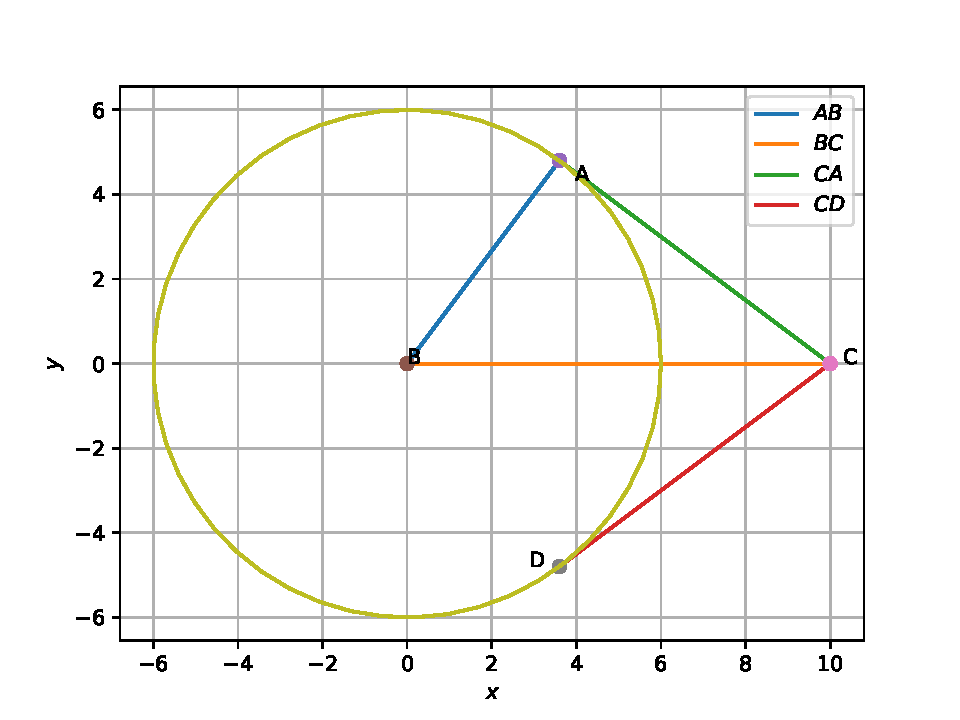
\includegraphics[scale=0.7]{circle}\\*
\line(1,0){350}\\*
{ If the correct matches are A-p,s and t;B-q and r; C-p and q and D-s then the correct darkening of bubbles will look like the given.}\\*
{1.Let the circles $C_1$\enspace:\enspace$x^2+y&2=9$ and $C_2\enspace:\enspace (x-3)^2+(y-4)^2=16$ intersect at points X and Y,suppose that another circle\\*
$C_3\enspace:\enspace (x-h)^2+(y-k)^2=\enspace r^2$ satisfies the following conditions\\*
(i)\enspace Center of $C_3$ is collinear with centre of $C_1$ and $C_2$\\*
(ii)\enspace $C_1$ and $C_2$ both lie inside $C_3$\\*
(iii)\enspace $C_3$ touches $C_1$ at M and $C_2$ at N\\*
Let the line through X and Y intersects $C_3$ at Z and at W, and let a common tangent of $C_1$ and $C_3$ be a tangent to the parabola $x^2$=8$\alpha$y\\*
\enspace There are some expressions given in the List-I whose values are given in List-II below.\\*}
{\Large\enspace\enspace\textbf{Column-I}\enspace\enspace\enspace\enspace\enspace\enspace\enspace\enspace\enspace\enspace\enspace\enspace\enspace\enspace\enspace\enspace\enspace\enspace\enspace\textbf{Column-II}\\*
}
{\Large\enspace\enspace(A)\enspace 2h+k\enspace\enspace\enspace\enspace\enspace\enspace\enspace\enspace\enspace\enspace\enspace\enspace\enspace\enspace\enspace\enspace\enspace\enspace\enspace\enspace\enspace\enspace(p)\enspace 6\\*
}
{\Large\enspace\enspace(B)\enspace ${\frac{length\enspace of\enspace ZW}{length\enspace of \enspace XY}}$\enspace\enspace\enspace\enspace\enspace\enspace\enspace\enspace\enspace\enspace\enspace\enspace\enspace\enspace\enspace\enspace(q)\enspace $\sqrt6$\\*
}
{\Large\enspace\enspace(C)\enspace ${\frac{Area\enspace of\enspace triangle\enspace MZN}{Area\enspace of \enspace triangle\enspace ZMW}}$\enspace\enspace\enspace\enspace\enspace\enspace\enspace\enspace\enspace\enspace(r)\enspace 5/4\\*
-\enspace\enspace\enspace\enspace\enspace\enspace\enspace\enspace\enspace\enspace\enspace\enspace\enspace\enspace\enspace\enspace\enspace\enspace\enspace\enspace\enspace\enspace\enspace\enspace\enspace\enspace\enspace\enspace\enspace\enspace(s)\enspace 21/5\\*
-\enspace\enspace\enspace\enspace\enspace\enspace\enspace\enspace\enspace\enspace\enspace\enspace\enspace\enspace\enspace\enspace\enspace\enspace\enspace\enspace\enspace\enspace\enspace\enspace\enspace\enspace\enspace\enspace\enspace(t)\enspace 2$\sqrt6$\\*
-\enspace\enspace\enspace\enspace\enspace\enspace\enspace\enspace\enspace\enspace\enspace\enspace\enspace\enspace\enspace\enspace\enspace\enspace\enspace\enspace\enspace\enspace\enspace\enspace\enspace\enspace\enspace\enspace\enspace\enspace(u)\enspace 10/3\\*
}
{Which of the following is the only CORRECT combination?}\\*
{\large (a)\enspace (I),\enspace(U)\\*
(b)\enspace (I),\enspace(S)\\*
(c)\enspace (II),\enspace(T)\\*
(d)\enspace (II),\enspace(Q)\\*
}
{1.Let the circles $C_1$\enspace:\enspace$x^2+y^2=9$ and $C_2\enspace:\enspace (x-3)^2+(y-4)^2=16$ intersect at the  points X and Y, suppose that another circle $C_3\enspace:\enspace (x-h)^2+(y-k)^2=\enspace r^2$ satsifies the following conditions\\*\\*
(i)\enspace Center of $C_3$ is collinear with centre of $C_1$ and $C_2$\\*
(ii)\enspace $C_1$ and $C_2$ both lie inside $C_3$\\*
(iii)\enspace $C_3$ touches $C_1$ at M and $C_2$ at N\\*
Let the line through X and Y intersects $C_3$ at Z and at W, and let a common tangent of $C_1$ and $C_3$ be a tangent to the parabola $x^2$=8$\alpha$y\\*
\enspace There are some expressions given in the List-I whose values are given in List-II below.\\*}
{\Large\enspace\enspace\textbf{Column-I}\enspace\enspace\enspace\enspace\enspace\enspace\enspace\enspace\enspace\enspace\enspace\enspace\enspace\enspace\enspace\enspace\enspace\enspace\enspace\textbf{Column-II}\\*
}
{\Large\enspace\enspace(A)\enspace 2h+k\enspace\enspace\enspace\enspace\enspace\enspace\enspace\enspace\enspace\enspace\enspace\enspace\enspace\enspace\enspace\enspace\enspace\enspace\enspace\enspace\enspace\enspace(p)\enspace 6\\*
}
{\Large\enspace\enspace(B)\enspace ${\frac{length\enspace of\enspace ZW}{length\enspace of \enspace XY}}$\enspace\enspace\enspace\enspace\enspace\enspace\enspace\enspace\enspace\enspace\enspace\enspace\enspace\enspace\enspace\enspace(q)\enspace $\sqrt6$\\*
}
{\Large\enspace\enspace(C)\enspace ${\frac{Area\enspace of\enspace triangle\enspace MZN}{Area\enspace of \enspace triangle\enspace ZMW}}$\enspace\enspace\enspace\enspace\enspace\enspace\enspace\enspace\enspace\enspace(r)\enspace 5/4\\*
-\enspace\enspace\enspace\enspace\enspace\enspace\enspace\enspace\enspace\enspace\enspace\enspace\enspace\enspace\enspace\enspace\enspace\enspace\enspace\enspace\enspace\enspace\enspace\enspace\enspace\enspace\enspace\enspace\enspace\enspace(s)\enspace 21/5\\*
-\enspace\enspace\enspace\enspace\enspace\enspace\enspace\enspace\enspace\enspace\enspace\enspace\enspace\enspace\enspace\enspace\enspace\enspace\enspace\enspace\enspace\enspace\enspace\enspace\enspace\enspace\enspace\enspace\enspace(t)\enspace 2$\sqrt6$\\*
-\enspace\enspace\enspace\enspace\enspace\enspace\enspace\enspace\enspace\enspace\enspace\enspace\enspace\enspace\enspace\enspace\enspace\enspace\enspace\enspace\enspace\enspace\enspace\enspace\enspace\enspace\enspace\enspace\enspace\enspace(u)\enspace 10/3\\*
}
{Which of the following is the only CORRECT combination?}\\*
{\large (a)\enspace (IV),\enspace(S)\\*
(b)\enspace (I),\enspace(P)\\*
(c)\enspace (III),\enspace(R)\\*
(d)\enspace (IV),\enspace(U)\\*
}\\*\\*
{\LARGE\enspace\textbf{Comprehension Based Questions}}}
{\Large\begin{center}
    {PASSAGE-1}
\end{center}} \\*\\
ABCD is square of side length 2 units.C1 is the circle touching all the sides of the square ABCD and C2 is the circumcircle of square ABCD.L is a fixed line in the same plane and R is a fixed point.\\*
1. If P is any point of C1 and Q is another point on C2 then\\*$PA^2+PB^2+PC^2+PD^2$/ $QA^2+QB^2+QC^2+QD^2$ is equal to\\*

\choice (a) 0.75

\choice (b) 1.25

\choice (c) 1

\choice (d) 0.5

2.If a circle is such that it touches the line L and the circle C1 externally,such that both the circles are on the same side of the line, then the locus of centre of circle is\\*

\choice (a) ellipse 

\choice (b) hyperbola

\choice (c) parabola

\choice (d) pair of straight line\\*

3. A line L' through A is drawn parallel to BD.Point S moves such that its distance from the line BD and the vertex A arc equal.If locus of S cuts L' at T2 and T3 and AC at T1, then area of triangle T1T2T3 is\\*\\*

\choice (a)1/2 sq.units

\choice (b) 2/3 sq.units

\choice (c) 1 sq.units

\choice (d) 2 sq.units\\*\\*

{\LARGE PASSAGE-2}\\*\\
 A circle C of radius 1 is inscribed in an equilateral triangle PQR,The points of contact of C with the sides PQ,QR,RP are D,E,F respectively.The line PQ is given by the equation  
\sqrt{3}x+y-6=0 \enspace and point D is (3\sqrt{3}/2,3/2) $Further,it is given that the origin and the center of C are on the same side of the line PQ.$\\*\\*

4. The equation of the circle C is \\*\\*

\choice (a) (x-2\sqrt{3})^2+(y-1)^2=1

\choice (b) (x-2\sqrt{3})^2+(y+1/2)^2=1

\choice (c) (x-\sqrt{3})^2+(y+1)^2=1

\choice (d) (x-\sqrt{3})^2+(y-1)^2=1\\*\\*

5.Points E and F are given by\\*\\*

\choice (a) (\sqrt{3}/2,3/2),(\sqrt{3},0)

\choice (b) (\sqrt{3}/2,1/2),(\sqrt{3},0)

\choice (c) (\sqrt{3}/2,3/2),(\sqrt{3}/2,1/2)

\choice (d) (3/2,\sqrt{3}/2),(\sqrt{3}/2,1/2) \\*\\*

6.\enspace Equation of the sides QR,RP are\\*\\*

\choice (a) y=(2/\sqrt{3})x+1,y=(-2/\sqrt{3})x-1

\choice (b) y=(1/\sqrt{3})x,y=0

\choice (c) y=(\sqrt{3}/2)x+1,y=(\sqrt{3}/2)x-1

\choice (d) y=\sqrt{3}x,y=0\\*\\*

{\LARGE PASSAGE-3}\\*\\*

 A tangent PT is drawn to the circle $x^2+y^2=4$ at the point P(\sqrt{3},1).\enspace$A straight line L,Perpendicular to PT is a tangent to the circle(x-3)^2+y^2=1.$\\*\\*

7.A possible equation of L is \\*\\*

\choice (a) x-\sqrt{3}y=1

\choice (b) x-\sqrt{3}y=1

\choice (c) x-\sqrt{3}y=1

\choice (d) x-\sqrt{3}y=1\\*\\

8.\enspace A common tangent of the two circles is\\*\\

\choice (a) x=4

\choice (b) y=2

\choice (c) x+\sqrt{3}y=4

\choice (d) x+2\sqrt{2}y=6\\*\\

{\LARGE PASSAGE-4}\\*\\*

 Let S be the circle in the xy-plane defined by the equation  x^2+y^2=4$\\*

9. Let E1 E2 and F1 F2 be the chords of S passing through the point P0(1,1) and Parallel to the x-axis and the y-axis respectively.Let G1G2 be the chord of S passing through P0 and having slope -1.Let the tangent to S at F1 and F2 meet at F3,and the tangent to S at G1 and G2 meet at G3.Then,the points E3,F3 and G3 lie on the curve$\\*\\*
 
 \choice (a) x+y=4

\choice (b) (x-4)^2+(y-4)^2=16

\choice (c) (x-4)(y-4)=4

\choice (d) xy=4\\*\\*

10.Let P be a point on the Circle S with both coordinates being positive.Let the tangent to S at P intersect the coordinate axes at the points M and N .Then,the mid-Point of the line segment MN must lie on the curve\\*\\*

\choice (a) (x+y)^2=3xy

\choice (b) x^(2/3)+y^(2/3)=2^(4/3)

\choice (c) x^2+y^2=2xy

\choice (d) x^2+y^2=x^2y^2\\*\\

{\LARGE Assertion and Reason Type Questions }\\*\\
1. Tangent are drawn from the point (17,7) to the circle x^2+y^2=169\\*
{\LARGE $STATEMENT-1$ }:\enspace $the tangents are mutually perpendicular because$\\*\\
{\LARGE $STATEMENT-2$ }:\enspace $The locus of the point from which mutually perpendicular tangents can be draw to the given circle $x^2+y^2=338$ \\*\\

\choice (a) Statement-1 is True,Statement-2 is True;Statement-2 is correct explanation for Statement-1

\choice (b) Statement-1 is True,Statement-2 is False;Statement-2 is NOT correct explanation for Statement-1

\choice (c) Statement-1 is True,Statement-2 is False 

\choice (d) Statement-1 is False,Statement-2 is True\\*\\*



2. Consider L1:2x+3y+p-3=0,L2:2x+3y+p+3=0 where P is a real number, and C:x^2+y^2+6x-10y+30=0.\\*\\*
{\LARGE $STATEMENT-1$ }:\enspace $If line L1 is a chord of circle C,Then line L2 is not always a diameter of circle C$\\*\\*
{\LARGE $STATEMENT-2$ }:\enspace $If line L1 is a diameter of circle C,Then line L2 is not a chord of circle C$\\*\\*

\choice (a) Statement-1 is True,Statement-2 is True;Statement-2 is correct explanation for Statement-1

\choice (b) Statement-1 is True,Statement-2 is False;Statement-2 is NOT correct explanation for Statement-1

\choice (c) Statement-1 is True,Statement-2 is False 

\choice (d) Statement-1 is False,Statement-2 is True\\*\\*
{\LARGE Integer Value Correct Type }\\*\\
1.The Center of two Circles C1 and C2 each of Unit radius are at a distance of 6 units from each other.Let P be the mid point of the line segment joining the centers of C1 and C2 and C be the circle touching circle C1 and C2 externally.if a common tangent to C1 and C passing through P is also a common tangent to C2 and C, then the radius of circle C is\\*\\*
2.The straight line 2x-3y=1 divides the circular region $x^2+y^2<=6$ into two parts.If S={{(2,3/4),(5/2,3/4),(1/4,1/4),(1/8,1/4)}} then number of points(s) in S lying inside the smaller part is\\*\\*
3. For how many values of p,the circle $x^2+y^2+2x+4y-p=0$ and the coordinate axes have exactly three common points?\\*\\*
4. Let point B be the reflection of the point A(2,3) with respect to the line 8x-6y-23=0.Let Ta and Tb be circles of radii 2 and 1 with centers A and B respectively.Let T be a common tangent to a circle Ta and Tb such that both the circles are on the same side of T.If C is the point of intersection of T and the line passing through A and B,then the length of the line segment AC is \\*\\*

{\LARGE SECTION-B }\\*

1. If the chord y=mx+1 of the circle $x^2+y^2=1$ subtends an angle of measure 45° at the major segment of the circle then value of m is\\*\\

\choice (a) 2\pm\sqrt{2}

\choice (b) -2\pm\sqrt{2}

\choice (c) -1\pm\sqrt{2}

\choice (d) none of these\\*\\*
2. The centers of set points of a circles,each of radius 3,lie on the circle $x^2+y^2=25$.the locus of any point in the set is\\*

\choice (a) 4\leq x^2+y^2 \leq 64

\choice (b)  x^2+y^2 \leq 25

\choice (c) x^2+y^2 \geq 25

\choice (d) 3\leq x^2+y^2 \leq 9\\*

3. The center of the circle passing through (0,0) and (1,0) and touching the circle $x^2+y^2=9$ is\\*

\choice (a) (1/2,1/2)

\choice (b) (1/2,-\sqrt{2})

\choice (c) (3/2,1/2)

\choice (a) (1/2,3/2)\\*

4. the equation of a circle with origin as a center passing through equilateral triangle whose median is of length 3a is\\*

\choice (a) x^2+y^2=9a^2

\choice (b) x^2+y^2=16a^2

\choice (c) x^2+y^2=4a^2

\choice (d) x^2+y^2=a^2

5. If the two circles $(x-1)^2+(y-3)^2=r^2$ and $x^2+y^2-8x+2y+8=0$ intersecting in two distinct point, then\\*

\choice (a) $r > 2$

\choice (b) $2< r < 8$

\choice (c) $ r < 2$

\choice (d) r=2\\*
6.The lines 2x-3y=5 and 3x-4y=7 are diameters of a circle having area as 154 sq.units. then the equation of the circle is\\*

\choice (a) $x^2+y^2-2x+2y=62$ 

\choice (b) $x^2+y^2+2x-2y=62$ 

\choice (c) $x^2+y^2+2x-2y=47$ 

\choice (d) $x^2+y^2-2x+2y=47$ \\*

7. if a circle passes through a point (a,b) and cuts the circle $x^2+y^2=4$ orthogonally then the locus of its center is\\*
\choice (a) 2ax-2by-(a^2+b^2+4)=0

\choice (b) 2ax+2by-(a^2+b^2+4)=0

\choice (c) 2ax-2by+(a^2+b^2+4)=0

\choice (d) 2ax+2by+(a^2+b^2+4)=0\\*

8.A variable circle passes through the fixed point A(p,q) and touches x-axis.the locus of the other end of the diameter through A is\\*

\choice (a) (y-q)^2=4px

\choice (b) (x-q)^2=4py

\choice (c) (y-p)^2=4qx

\choice (d) (x-p)^2=4qy\\*

9. If the lines 2x+3y+1=0 and 3x-y-4=0is lie along diameter of a circle of circumference 10$\pi$,then the equation of the circle is\\*
\choice (a) $x^2+y^2+2x-2y-23=0$ 

\choice (b) $x^2+y^2-2x-2y-23=0$ 

\choice (c) $x^2+y^2+2x+2y-23=0$ 

\choice (d) $x^2+y^2-2x+2y-23=0$ \\*

10.Intercept on the line y=x by the circle $x^2+y^2+2x$=0 is AB.Equation of the circle on AB as a diameter is\\*

\choice (a) $x^2+y^2+x-y=0$ 

\choice (a) $x^2+y^2-x+y=0$ 

\choice (a) $x^2+y^2+x+y=0$ 

\choice (a) $x^2+y^2-x-y=0$ \\*

11. if the circle $x^2+y^2+2ax+cy+a=0$ and $x^2+y^2-3ax+dy-1=0$ intersect in two distinct points P and Q then the lines 5x-by-a=0 passes through P and Q for\\*

\choice (a) exactly one value of a 

\choice (b) no value of a 

\choice (c) infinitely many values of a

\choice (d) exactly two values of a\\*

12. A circle touches the x-axis and also touches the circle with centre at (0,3) and radius 2.The locus of the centre of the circle is\\*

\choice (a) an ellipse

\choice (b) a circle 

\choice (c) a hyperbola

\choice (d) a parabola\\*

13.if a circle passes through the point (a,b) and cuts the circle $x^2+y^2=p^2$ orthogonally, then the equation of the locus of its center is\\*

\choice (a) $x^2+y^2-3ax-4by+(a^2+b^2-p^2)=0

\choice (b) 2ax+2by-(a^2-b^2+p^2)=0

\choice (c) $x^2+y^2-2ax-3by+(a^2-b^2-p^2)=0

\choice (d) 2ax+2by-(a^2+b^2+p^2)=0\\*

14.if the lines $ax^2+2(a+b)xy+by^2=0$ lie along diameters of a circle and divide the circle into four sectors such that the area of one of the sectors is thrice the area of another sector then\\*

\choice (a) 3a^2-10ab+3b^2=0

\choice (a) 3a^2-2ab+3b^2=0

\choice (a) 3a^2+10ab+3b^2=0

\choice (a) 3a^2+2ab+3b^2=0\\*

15. if the lines 3x-4y-7=0 and 2x-3y-5=0 are two diameters of a circle of area 49$\pi$ sq.units,the equation of the circle is\\*

\choice (a) $x^2+y^2-2x-2y-47=0$ 

\choice (b) $x^2+y^2+2x-2y-62=0$ 

\choice (c) $x^2+y^2-2x+2y-62=0$ 

\choice (d) $x^2+y^2-2x+2y-47=0$ \\*

16. let C be the circle with center (0,0) and radius 3 units.the equation of the locus of the mid points of the chords of the circle C that subtend angle of 2$\pi$/3 at its center is\\*

\choice (a) $x^2+y^2=3/2$

\choice (b) $x^2+y^2=1$

\choice (c) $x^2+y^2=27/4$

\choice (d) $x^2+y^2=9/4$\\*

17. Consider a family of circles which are passing through the points (-1,1) and are tangent to x-axis.if (h,k) are the coordinates of the centre of the circles,then the set of values of k given by the interval\\*

\choice (a) -1/2\leq k\leq1/2

\choice (b)  k\leq1/2

\choice (c) 0\leq k\leq1/2

\choice (d) k\geq1/2\\*

18. the point diametrically opposite to the point P(1,0) on the circle $x^2+y^2+2x+4y-3=0$ is

\choice (a) (3,-4)

\choice (b) (-3,4)

\choice (c) (-3,-4)

\choice (d) (3,4)\\*

19. the differential equation of family of circles with fixed radius 5 units and center on the line y=2 is\\*

\choice(a) $(x-2)y^2=25-(y-2)^2$

\choice(b) $(y-2)y^2=25-(y-2)^2$

\choice(c) $(y-2)^2y^2=25-(y-2)^2$

\choice(d) $(x-2)^2y^2=25-(y-2)^$\\*

20. if P and Q are the points of intersection of the circles $x^2+y^2+3x+7y+2p-5=0$ and $x^2+y^2+2x+2y-p^2=0$ then there is a circle passing through P,Q and (1,1) for\\*

\choice (a) all except one value of p

\choice (b) all except two values of p

\choice (c) exactly one value of p

\choice (d) all values of p\\*

21. the circle $x^2+y^2=4x+8y+5$ intersects the line 3x-4y=m at two distinct points if\\*

\choice (a) -35$<$m$<$15

\choice (b) 15$<$m$<$65

\choice (c) 35$<$m$<$85

\choice (d) -85$<$m$<$-35\\*

22. The two circles $x^2+y^2=ax$ and $x^2+y^2=c^2$ C$>$0 touch each other if\\*

\choice (a) \mid a\mid=c

\choice(b) a=2c

\choice (c) \mid a\mid=2c

\choice (d) 2\mid a\mid=c\\*

23. the length of the diameter of the circle which touches the x-axis at the point (1,0) and passes through the point (2,3) is \\*

\choice (a) 10/3

\choice (b) 3/5

\choice (c) 6/5

\choice (d) 5/3\\*

24. the circle passing through (1,-2)and touching the axis of x at (3,0) also passes through the point\\*

\choice (a) (-5,2)

\choice (b) (2,-5)

\choice (c) (5,-2)

\choice (d) (-2,5)\\*

25. Let C be the circle with center (1,1) and radius =1.If T is the circle centred at (0,y),passing through origin and touching the circle C externally, then the radius of T is equal to\\*

\choice (a) 1/2

\choice (b) 1\4

\choice (c) \sqrt{3}/\sqrt{2}

\choice (d)\sqrt{3}/2\\*

26.Locus of the image of the point (2,3) in the line (2x-3y+4)+k(x-2y+3)=0, k\in R is a\\*

\choice (a) circle of radius \sqrt{2}

\choice (b) circle of radius \sqrt{3}

\choice (c) straight line parallel to x-axis

\choice (d) straight line parallel to y-axis\\*

27. the number of common tangents to the circles   $x^2+y^2-4x-6y-12=0$ and $x^2+y^2+6x+18y+26=0$ is\\*

\choice (a) 3

\choice (b) 4

\choice (c) 1

\choice (d) 2\\*

28. the centers of those circles which touches the circle $x^2+y^2-8x-8y-4=0$ externally and also touches the x-axis lie on\\*

\choice (a) an parabola

\choice (b) a circle 

\choice (c) a hyperbola

\choice (d) a ellipse which is not a circle\\*

29.if one of the diameter of the circle given by the equation $x^2+y^2-4x+6y-12=0$  is a chord of a circle S, whose centre is at (-3,2), then the radius of S is\\*

\choice (a) 5

\choice (a) 10

\choice (a) 5\sqrt{2}

\choice (a) 5\sqrt{3}\\*

30. if the tangent to the circle $x^2+y^2=1$ intersects the coordinates axes at distinct points P and Q, then the locus of the mid-point of PQ is\\*

\choice (a) $x^2+y^2-4x^2y^2=0$

\choice (b) $x^2+y^2-2xy=0$

\choice (c) $x^2+y^2-16x^2y^2=0$

\choice (d) $x^2+y^2-2x^2x^2=0$
\end{document}
